%\NeedsTeXFormat{LaTeX2e} 		%???

\documentclass[notheorems,12pt]{beamer}

\usepackage[czech]{babel}
\usepackage[utf8]{inputenc}
\usepackage[T1]{fontenc}
\usepackage{enumerate,epsf,colortbl,color,colordvi}
\usepackage{graphicx, float}
\usepackage{subfig} 	%subfloats.

\usetheme{metropolis}
\metroset{numbering=none}
%\usetheme{Berlin}
\usecolortheme{beaver}

\setbeamertemplate{itemize items}[square]
\setbeamertemplate{theorems}[numbered]

\usepackage{graphicx}
\usepackage{amsmath}							% great math stuff
\usepackage{amsfonts}							% for blackboard bold, etc
\usepackage{amsthm}								% better theorem environments
\usepackage{amssymb}

\usepackage{units}
\usepackage{physics}
\usepackage{subfig} 	%subfloats.
\captionsetup[subfigure]{labelformat=empty} %odstrani (a), (b),... u subfloats

\usepackage{caption} %abych mohl pouzit \caption*{•}

\usefonttheme[onlymath]{serif} 	%dela peknou matematiku ;)


\nonumber
\title[]{\#filterbubble}
\date{}
\author{Františka Sandroni\\
        Jakub Dostál}
\institute{}
% ############################################
% ############################################
\begin{document}
\maketitle
% ############################################
% ############################################
\begin{frame}{Filter bubble}
\begin{itemize}
    \item Eli Pariser - 2011
    \item sociální sítě
    \item preferenční algoritmy
\end{itemize}
\end{frame}
% ############################################
% ############################################
\begin{frame}{Důsledky}
\begin{columns}
	\column{6cm}
	\begin{block}{Negativní}
		\begin{itemize}
			\item heterogenita
            \item ztráta objektivity
            \item radikalizace
            \item ohrožení demokracie
		\end{itemize}
	\end{block}
	\column{6cm}
	\begin{block}{Positivní}
		\begin{itemize}
			\item personalizace
            \item cílená informovanost
            \item úspora času
		\end{itemize}
	\end{block}
\end{columns}
\end{frame}
% ############################################
% ############################################
\begin{frame}{Sentimentální analýza}
\begin{itemize}
    \item machine learning, big data
    \item klasifikace
    \item positivní vs. negativní text
\end{itemize}
\end{frame}
% ############################################
% ############################################
\begin{frame}{Twitter}
    \begin{columns}
    \column{5cm}
    	\begin{itemize}
    		\item sociální síť
    		\item informační kanál
    		\item \# hashtag
    		\item following, followers
    	\end{itemize}
    \column{6cm}
    	\center
    	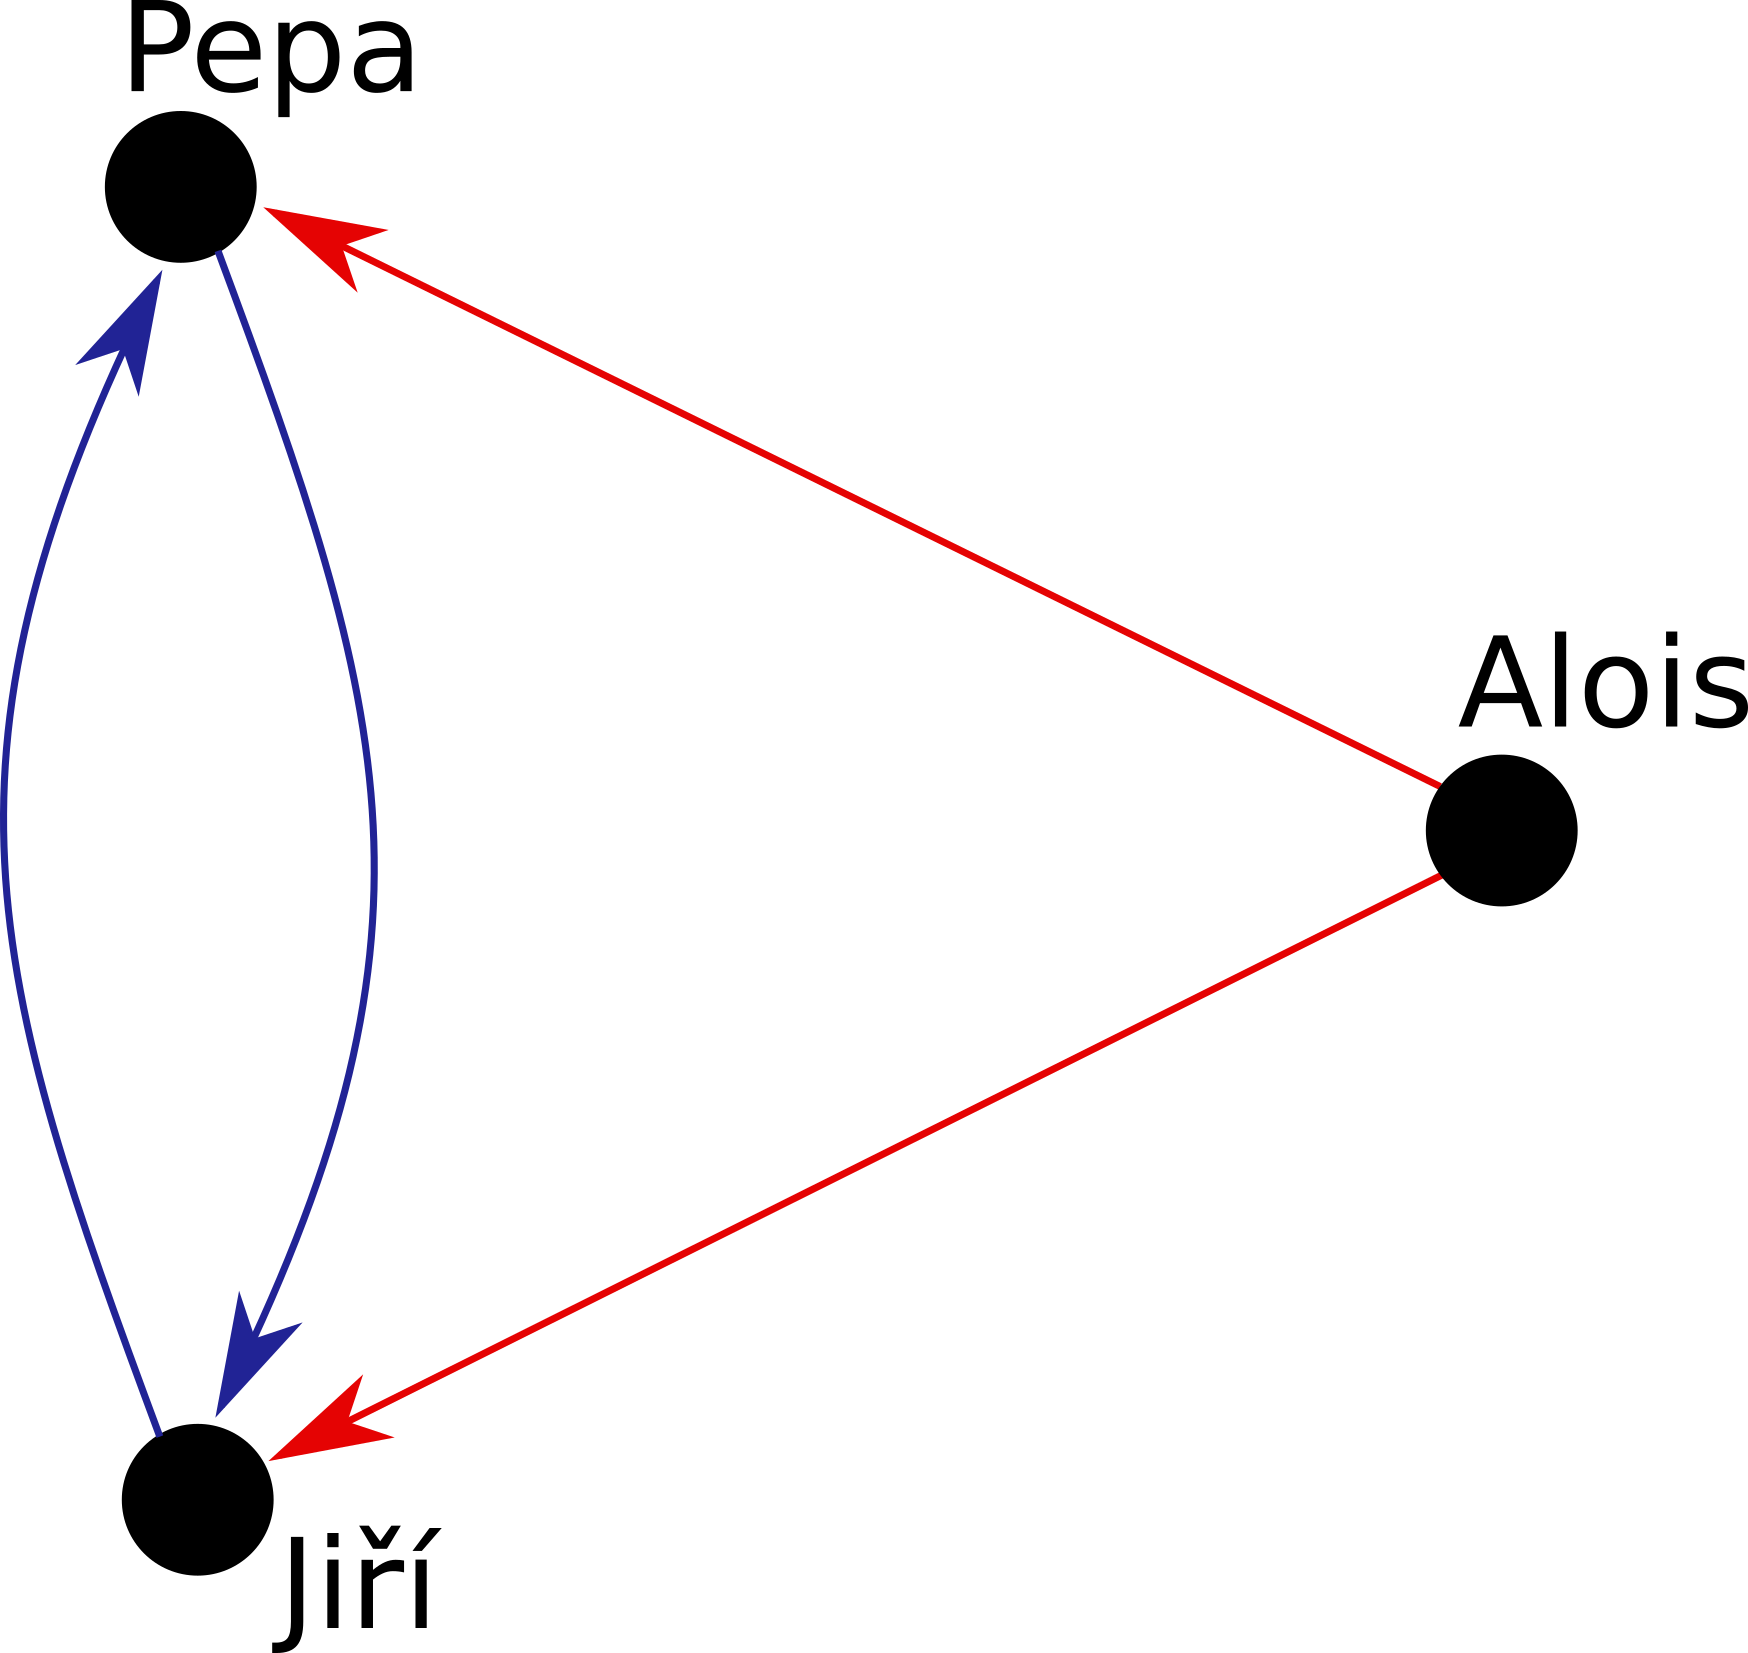
\includegraphics[scale=0.35]{./Pics/pepa.png}
    \end{columns}
\end{frame}
% ############################################
% ############################################
\begin{frame}{Konstrukce měření}
    \begin{columns}
    \column{5cm}
    	\begin{itemize}
    		\item pozorované skupiny
    		\item okolí uživatele
    		\item klíčové slovo
    		\item \textit{large scale} experiment
    	\end{itemize}
    \column{6cm}
    	\center
    	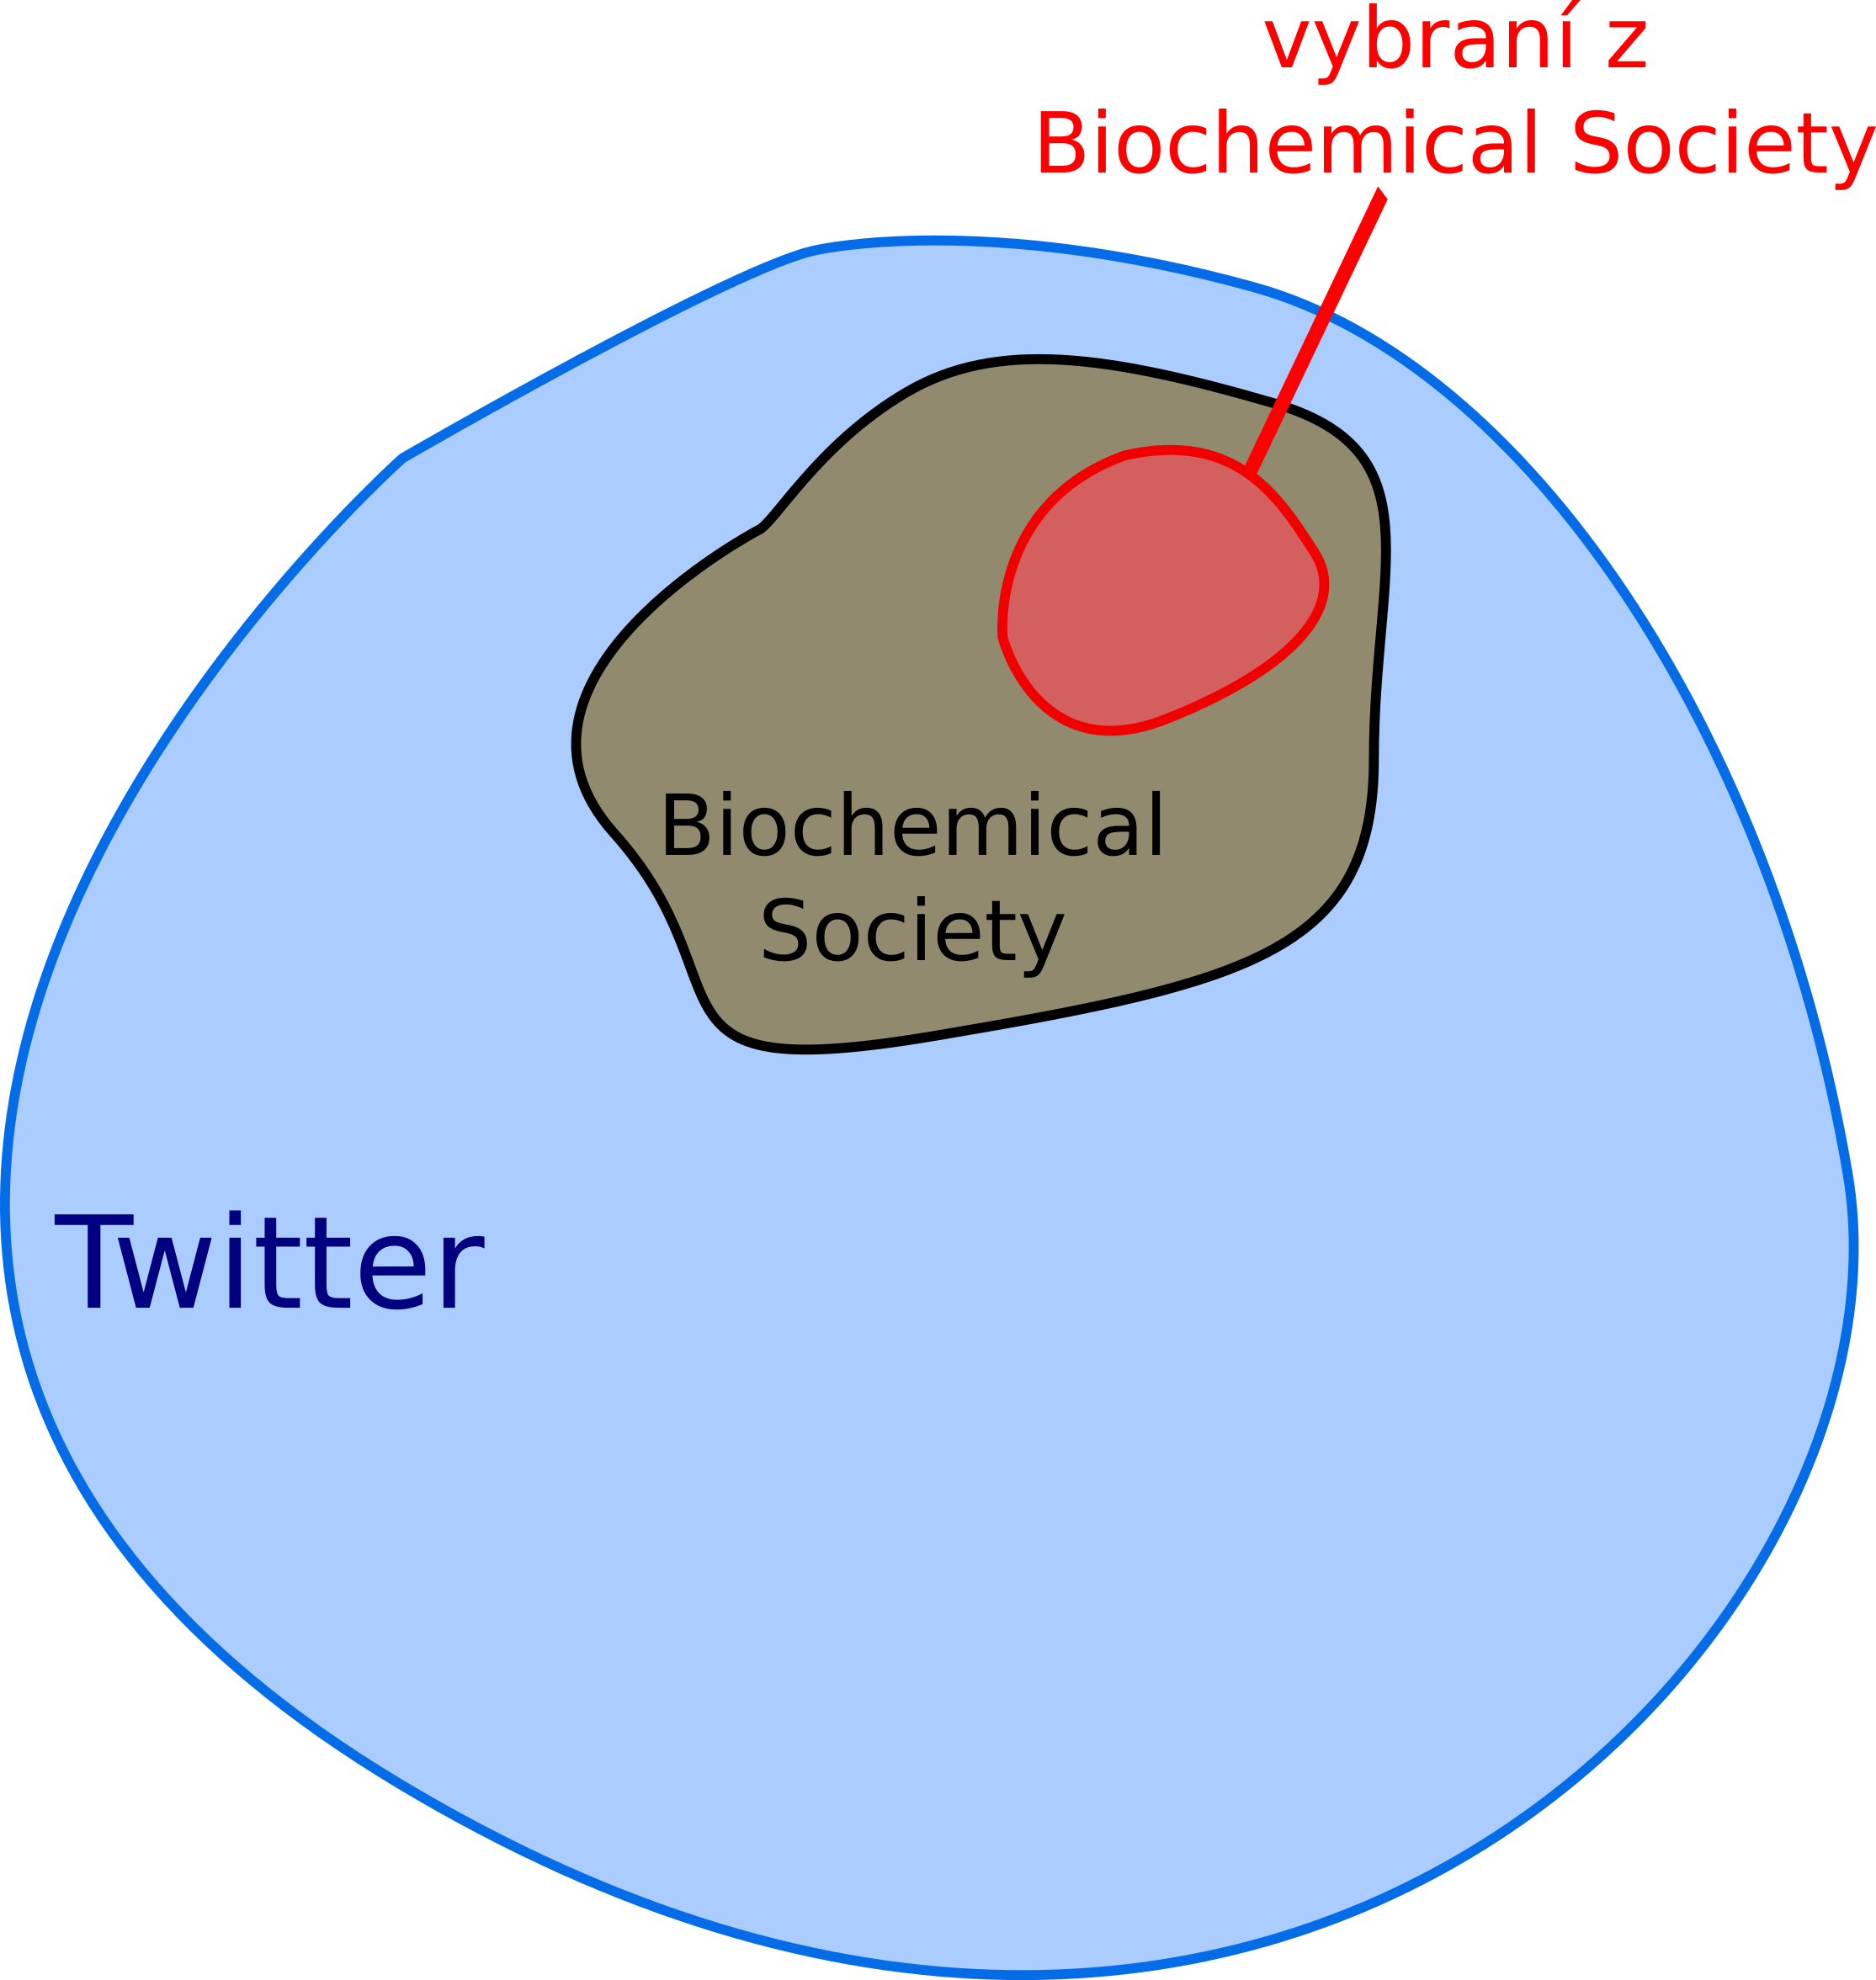
\includegraphics[scale=0.32]{./Pics/sets.png}
    \end{columns}
\end{frame}

% ############################################
% ############################################
\end{document}
